\documentclass[class=scrartcl, crop=false]{standalone}

\usepackage[sexy]{evan}
\usepackage{cole}

\graphicspath{ {./images/} }

\date{2020-05-06}


\begin{document}

\section{05-06}

\subsection{Minimization of DFA}

Example of machine that checks divisibility by 3. But we already saw a three state machine that does the same thing.

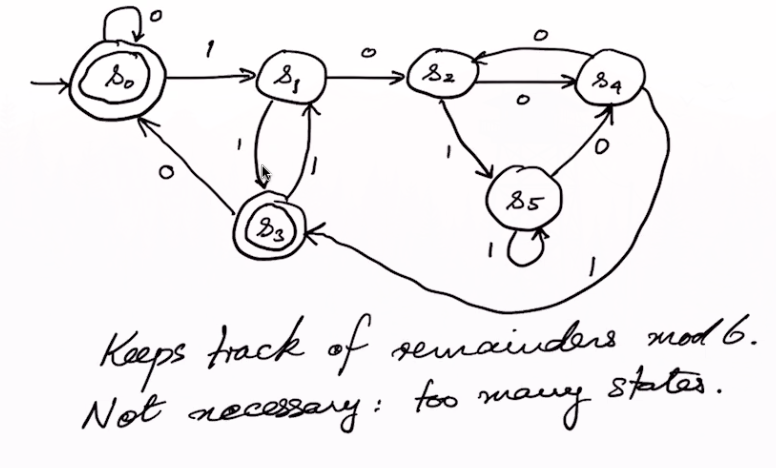
\includegraphics[width=\textwidth]{mod6machine}
\begin{gather*}
  \delta(s_0, 0) = s_0 = \delta(s_3, 0)
  \delta(s_1, 1) = s_1 = \delta(s_3, 1)
\end{gather*} 
These states are doing the same thing so there's no reason to keep them separate.
\begin{note}
  Once you get to a state, it doesn't matter how you got there. What happens in the future only depends on what you read in the future.
  \\\\
  This is the fundamental meaning of the word state. It encodes the information to predict the future.
\end{note} 
\begin{definition}
  Given a DFA $M = (S, s_0, \delta, F)$, $\Sigma, p, q$ are \ul{equivalent}, $p \approx q$ if 
  \begin{gather*}
    \forall x \in \Sigma^*, \ \delta^*(p, x) \in F \Leftrightarrow \delta^*(q, x) \in F
  \end{gather*} 
  So the languages defined by their starting states are the same.
  \begin{remark}
    $p \not\approx q$ means $\exists x \in \Sigma^*$ such that 
    \begin{gather*}
      (\delta^*(p, x) \in F \ \wedge \ \delta^*(q, x) \notin F) \\
      \vee
      \\
      (\delta^*(p, x) \notin F \ \wedge \ \delta^*(q, x) \in F)
    \end{gather*} 
  \end{remark} 
  Observe that $\approx$ is an equivalence relation.
\end{definition} 

\begin{lemma}
  ghi
  % $p \approx q \Rightarrow \forall a \in \Sigma \ \delta(p, a) \approx \delta(q, a)$. But not necessarily $\delta(p, a) = \delta(q, a)$.
  % \begin{gather*}
  %   hi
  %   % [p] \coloneqq \{q \ | \ p \approx q\}, \ p \approx q \Leftrightarrow [p] = [q]
  % \end{gather*} 
  % \\\\
  % This means that $[p] = [q] \Rightarrow [\delta(p, a)] = [\delta(q, a)]$.
\end{lemma} 

We define a new machine $M' = (S', s_0', \delta', F')$. 

\begin{gather*}
  S' % = S / \approx, \ s_0' = [s_0], \ F'\{[s] \ \} % revisit
\end{gather*} 
This is a simpler dfa

\begin{lemma}
  \begin{gather*}
    
   p \in F \ \wedge p \approx q \Rightarrow q \in F
  \end{gather*} 
  This is trivial when considering $\epsilon \in \Sigma^*$

\end{lemma} 
\begin{lemma}
  $\forall w \in \Sigma^*, \ \delta'^*([p], w) = [\delta^*(p, w)]$
  \begin{proof}
    By induction on the length $w$.
  \end{proof}
\end{lemma} 

\begin{theorem}
  $L(M) = L(M')$
  \begin{proof}
    \begin{gather*}
      x \in L(M') \Leftrightarrow \delta'^*([s_0], x) \in F' \\
      \Leftrightarrow [\delta^*(s_0, x)] \in F' \Leftrightarrow \delta^*(s_0, x) \in F \\
      \Leftrightarrow x \in L(M)
    \end{gather*} 
  \end{proof} 
  Quotient construction. Might be that every equivalence class contains element, but maybe each one contains several states. But definitely didn't get a bigger machine. This process is called collapsing a machine.
\end{theorem} 

\subsection{Splitting Algorithm}

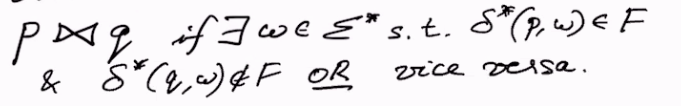
\includegraphics[width=\textwidth]{splittingalgorithm}

\begin{fact}
  If $\exists a \in \Sigma$ such that $\delta(p, a) bowtie \delta(q, a)$, then $p bowtie q$. The contrapositive of the above.
\end{fact} 

Matrices of booleans. You can multiply matrices of booleans by using "and" and "or". The collection of $n \times n$ matrices over a ring is always a ring.
\\\\
Algorithm
\begin{enumerate}
  \ii
  For every $(p, q)$ such that $p \in F \wedge q \notin F$, put $0$ in the $(p, q)$ cell of the matrix.
  \ii
  Repeat until no more changes. For each pair $(p, q)$ that is not already marked with a 0, check if $\exists a \in \Sigma$ such that $(\delta(p, a), \delta(q, a))$ is marked with 0. If so mark $(p, q)$ 0.
\end{enumerate} 
This algorithm correctly computes the equivalence classes. The time complexity is $O(n^4)$ in the naive case. $O(n^2k)$ using data structures. $O(n\log n)$ Hopcraft method.

\begin{theorem}
  If at the end two states are not marked 0 then they are equivalent.
\end{theorem} 

\begin{theorem}
  There is a unique minimal automaton to recognize a regular language.
  \\\\
  This is how you prove the equivalence of regular expressions.
\end{theorem} 

\begin{definition}[Right invariant]
  An equivalence relation $R$ on $\Sigma^*$ is said to be \ul{right-invariant} if 
  \begin{gather*}
    \forall x, y \in \Sigma^* \ \text{such that} \ xRy \Rightarrow \forall z \in \Sigma^*, \ azRyz
  \end{gather*} 
  \begin{example}
    DFA $M = (Q, \Sigma, q_0, \delta, F)$,
    \begin{gather*}
      xR_m y \Leftrightarrow \delta^*(q_0, x) = \delta^*(q_0, y)
    \end{gather*} 
  \end{example} 
  \begin{example}
    Given $L \subseteq \Sigma^*$, not necessarily regular, we define $R_L$ on $\Sigma^*$
    \begin{gather*}
      xR_Ly \Leftrightarrow xz \in L \Leftrightarrow yz \in L
    \end{gather*} 
  \end{example} 
\end{definition} 

\begin{note}
  The index of an equivalence relation is the number of equivalence classes. Infinite equivalency classes means infinite index.
\end{note} 

\begin{theorem}[Myhill-nerode 1957]
  The following are equivalent
  \begin{enumerate}
    \ii
    $L$ is regular
    \ii
    $L$ is the union of some of the equivalence classes of a right-invariant equivalence relation $R$ of finite index.
    \ii
    Any equivalence relation $R$ with the properties described in (2) has to refine $R_L$.
  \end{enumerate} 
  \begin{note}
    To say that an equivalence relation refines another means that it partitions all the equivalence relations.
  \end{note} 
  Full proof is in the notes.
\end{theorem} 

\subsection{Brozozowski's Algorithm}

Will convert some DFA to NFA. 

\begin{enumerate}
  \ii
  Reverse all the arrows change the initial states to an accept state, and make all the accept states start states.
  \ii
  Determinize it. This may cause exponential blow up because you are looking at the set of all subsets. Convert it from NFA to DFA.
  \ii
  Remove unreachable states.
  \ii
  Repeat 1.
  \ii
  Repeat 2. Might expect double exponential blow up, but instead there is a huge collapse to the minimal version of the original machine.
  \ii
  Repeat 3.
\end{enumerate} 
The result is the minimal machine.
\\\\
Can't explain the whole thing. The point is to get interested and excited about this topic.

\begin{note}
  $X^A$ means the set of all functions from $A$ to $X$. $\delta(x): X \to X^A$.
  \begin{gather*}
    X^A \approx [A \to X]
  \end{gather*} 
  We can either write $\delta(x)(a)$ in which case $\delta:X \to X^A$ or $\delta(x, a)$ where $\delta: X \times A \to X$. This process is called currying. \\
  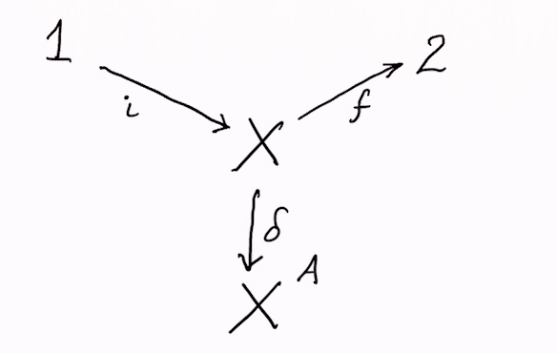
\includegraphics[width=\textwidth]{thisisanautomaton}
\end{note} 

\subsection{Infinite state automata}
$A^*$ is set of all words. Every word is a state. Initiale state is empty word.
\\\\
States are words. Transition is stick the new letter at the end of the word.
\\\\
There exists a \ul{unique} map $r: A^* \to X$ such that the diagram above commutes.
\\\\
Whatever path you follow that leads to the same end state results in the same outcome. Same as moving a different path with different endpoints.
\begin{note}
  Give $f: V \to W$, $f^A: V^A \to W^A$. $\varphi \in V^A$, then $f^A(\varphi)(a) = f(\varphi(v))$. This is countably infinite.
  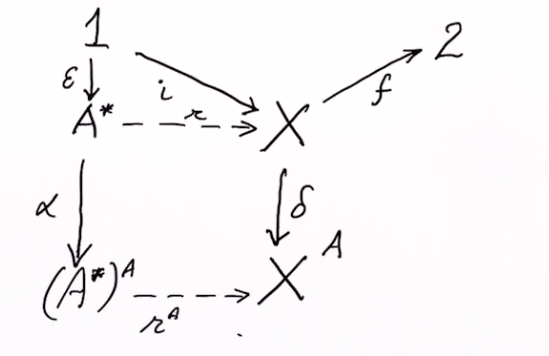
\includegraphics[width=\textwidth]{thisisanautomaton2}
  \begin{definition}[Reachability]
    $r$ maps the empty string to the . $r$ tracks every word through the automaton with $\delta^*$. $r$ is the \ul{reachability map}. It tells you which states can be reached. An automaton is reachable if every state can be reached.
  \end{definition} 
\end{note} 

\end{document}
